%% Copernicus Publications Manuscript Preparation Template for LaTeX Submissions %% ---------------------------------
%% This template should be used for copernicus.cls
%% The class file and some style files are bundled in the Copernicus Latex Package which can be downloaded from the different journal webpages.
%% For further assistance please contact the Copernicus Publications at: publications@copernicus.org
%% http://publications.copernicus.org
%% Please use the following documentclass and Journal Abbreviations for Discussion Papers and Final Revised Papers.
%% 2-Column Papers and Discussion Papers
\documentclass[gmd,dvipsnames]{copernicus}
\usepackage[table]{xcolor}% http://ctan.org/pkg/xcolor
\usepackage{lineno}
\usepackage{wrapfig}
\usepackage{graphicx}
\usepackage{framed}
\usepackage{hyperref}
\usepackage{tikz}
\usepackage{pdflscape}
\usepackage{afterpage}
\usepackage{csquotes}
\usepackage{booktabs}
\usepackage{siunitx}
\usepackage[shortlabels]{enumitem}
\sisetup{per-mode=reciprocal}
\DeclareSIUnit\kgC{kgC}

% can remove this before submission, only used so we can have sout during editing.
\usepackage[normalem]{ulem}
\usepackage{breakurl}


%% remove error warnings associated with bibtex typesetting of references.
\usepackage{etoolbox}
\apptocmd{\sloppy}{\hbadness 10000\relax}{}{}

%% hhline for double horizontal line
\usepackage{hhline}

% to keep tables to location where they are placed in the text.
\usepackage{float}
\restylefloat{table}

\hyphenation{experi-ments model-ling} 


%% for in-line code: https://tex.stackexchange.com/questions/19004/how-to-format-an-inline-source-code
\usepackage{listings}
\usepackage{color}
\definecolor{lightgray}{gray}{0.9}
\definecolor{llgray}{gray}{0.9}

\lstset{
    showstringspaces=false,
    basicstyle=\ttfamily,
    keywords={Tier 1, Tier 2},
    %keywordstyle=\color{blue},
    keywordstyle=\ttfamily,
    commentstyle=\color[grey]{0.6},
    breaklines=true,
    stringstyle=\ttfamily
}
    %%postbreak=\mbox{{$\hookrightarrow$}\space},

%%\newcommand{\code}[1]{\texttt{#1}}
%%\newcommand{\code}[2]{\colorbox{lightgray}{\lstinline[language=#1]$#2$}}
\lstdefinestyle{Inline}
{
          literate={\\-}{}{0\discretionary{-}{}{}}
}
\newcommand{\code}[2]{\lstinline[style=Inline,language=#1]$#2$}
\newcommand{\cd}[1]{\code{Python}{#1}}
\newcommand{\cdh}[1]{\lstinline[style=Inline,language=Python,postbreak=\mbox{{$\hookrightarrow$}\space}]$#1$}
\newcommand{\cdn}[1]{\lstinline[style=Inline,language=Python,breaklines=false]$#1$}
\newcommand\Tstrut{\rule{0pt}{2.6ex}} % top strut

% for table of contents
\usepackage{tocloft}

\cftsetindents{section}{0em}{2em}
\cftsetindents{subsection}{0em}{2em}

\renewcommand\cfttoctitlefont{\hfill\Large\bfseries}
\renewcommand\cftaftertoctitle{\hfill\mbox{}}

\setcounter{tocdepth}{2}

%% for "rowcolor" in tables .. for heading row. -- but conflicts with other usage.
%%\usepackage[table]{xcolor}

\usepackage{array,ragged2e}
\newcolumntype{R}[1]{>{\raggedleft\let\newline\\\arraybackslash\hspace{0pt}}m{#1}}

% 
%% added for UML
\usepackage{tikz-uml}
\usetikzlibrary{calc}
\usetikzlibrary{shapes}
%%%%%%%%%%%%%%%%%%%%%%%%%%%%
\usetikzlibrary{arrows,positioning,shapes.geometric}

%%\input{../maps/ice_sst3.htex}

\begin{document}

%% define new column type ... to avoid warnings on typesetting in paragraphs in table.
\newcolumntype{P}[1]{>{\raggedright\arraybackslash}p{#1}}

%% for plev table
\newlength{\xx}
\setlength{\xx}{4.2mm}
%%%%%%%%%%%%%%%%%%%%%%%%%%
\newcommand{\editorial}[1]{\textit{\color{red}#1}}
\newcommand{\response}[1]{\textit{\color{blue}#1}}

\renewcommand{\labelitemi}{$\bullet$}
\def\rot{\rotatebox}
\bibliographystyle{copernicus}
%%\bibliography{ams.bib}
\linenumbers
\title{A Registry for Data Specifications in Earth System Modelling}
\Author[1]{Martin}{Juckes}
%%\Author[2]{Karl E.}{Taylor}
%%\Author[2]{Paul}{Durack}
%%\Author[3]{Bryan}{Lawrence}
%%\Author[4]{Matthew}{Mizielinski}
%%\Author[1]{Alison}{Pamment}
%%\Author[5]{Jean-Yves}{Peterschmitt}
%%\Author[6]{Michel}{Rixen}
%%\Author[7]{St\'ephane}{S\'en\'esis}
%%\Author[]{}{}
\affil[1]{Science and Technology Facilities Council, Oxfordshire, UK}
%%\affil[2]{PCMDI, Lawrence Livermore National Laboratory, Livermore, DA, USA}
%%\affil[5]{IPSL}
%%\affil[7]{CNRM}
%%\affil[6]{WCRP}
%%\affil[3]{Uni. Reading}
%%\affil[4]{UK Met Office}
%% The [] brackets identify the author with the corresponding affiliation. 1, 2, 3, etc. should be inserted.
\runningtitle{DR Registry}
\runningauthor{Martin Juckes}
\correspondence{Martin Juckes (martin.juckes@stfc.ac.uk)}
\received{}
\pubdiscuss{} %% only important for two-stage journals
\revised{}
\accepted{}
\published{}
%% These dates will be inserted by Copernicus Publications during the typesetting process.
\firstpage{1}
\maketitle

\begin{abstract}
Establishing a registry to hold specifications of data variables and file formats for Earth System Models.
Based on principles established in the CMIP6 Data Request, designed to support a wider community.
\end{abstract}

\introduction  %% \introduction[modified heading if necessary]


\section{Context}
\label{s:history}

The CMIP6 Data Request specifies thousands of variables which are requested to support analysis of CMIP6 experiments.

The specifcations are provided in a technical document together with supporting software and web interfaces. 

The level of standardisation of data products within CMIP enables relatively easy use of the data by a broad community.

This paper describes the creation of a sustainable registry, which is designed to enable the registration
of technical specifications of variables by a broader community and also to streamline the process for CMIP.


The framework for registry organisational design set out in the ISO 19135 standard for geospatial registries
is adopted. This framework facilitates a clear separation of roles enabling efficient operation of the 
registry to support both the diverse requirements of the scientific domain and the diverse requirements of the 
science programme managers and governance bodies.


\subsection{Challenges}

The principle challenge comes from the need to support projects involving consortia of consortia (CCPs). Large consortium
projects may already be challenging when it is necessary to align practises of teams from many institutions, and the teams
in question may have many competing priorities outside the consortium. With a CCP, such as CMIP, the problems become 
far more challenging. Consortia may go through a long process to reach an agreement on some topic, only to find that an
independent consortium has adopted a conflicting approach. 

\section{Approach}

\subsection{Who is being supported}

The registry is primarily targetted at the Consortia of Consortia challenge, dealing with projects such as CMIP and CORDEX.

The {\bf domain} supported by the registry is research in the climate of the Earth system. Within this domain, there are communities 
establised around programmes such as CMIP and CORDEX. 

Within these communities there are multiple consortia, such as the MIPs in CMIP or the regional coordination groups in CORDEX.

The key point about these communities, which is essential for the functioning of the registry, is the existence of a governance body
which sets framework requirements for the information to be stored. 




\subsection{What is being managed}

A registry, following ISO19135, is considered as an organisation hosting registers. Each register is a collection of registered items of information, 
submitted by the scientific community. The register functions as a shared shared reference resource supporting the aims identified by the governance
group associated with the register.

The ability of the registry to support a range of registers with different governance groups is of critical importance. This ability
follows naturally from the ISO standard.

Different registers may have different submission criteria. Some may contain items which register information specific to the group 
submitting the information. In this case, the approval process need only look at the technical compliance of the information provided.

In other cases, the items are intended to be a shared resource. When a new item is proposed, there needs to be a community wide discussion 
to ensure that any addition is supported across the community.


\subsection{The Governance Framework}

The 

\subsection{The Operational Framework}

The operation of the registry is designed to provide a flexible platform to maintain and develop the registers.

\begin{figure*}[ht]
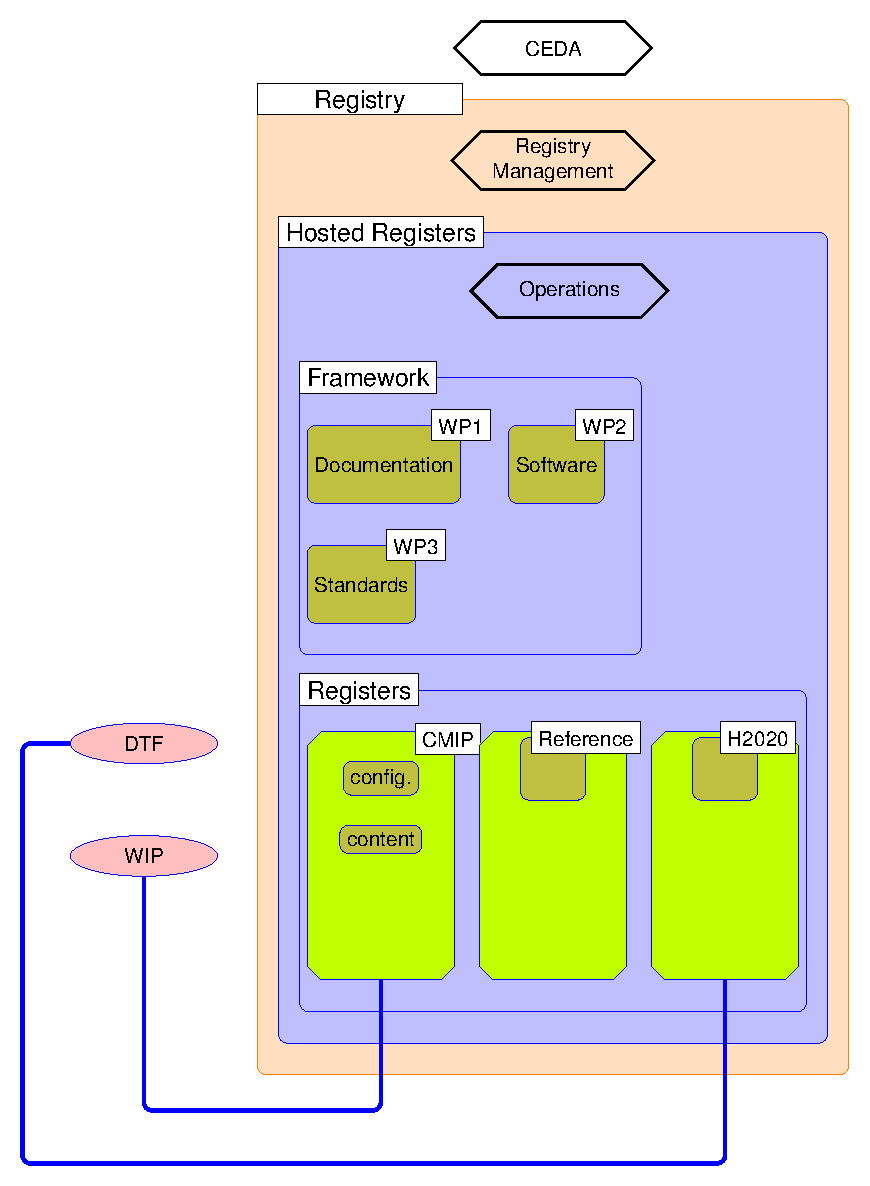
\includegraphics[width=8cm ]{../diagrams/reqreq01.pdf}
	\caption{
Organisational chart for the registry.
	}
	\label{fig:sketch}
\end{figure*}



%% START CONCLUSIONS ....

%\conclusions[Summary and Outlook]  %% \conclusions[modified heading if necessary]
% use a regular section during drafting to make viewing and navigating easier,
% change back to regular GMD style later.
\section{Summary and Outlook}
\label{s:end}


\subsection{Accessing the Registry}

The current version of the DREQ is available from the project website: 
\href{https://w3id.org/cmip6dr}{w3id.org/cmip6dr}
under the MIT License (BSD).
It is provided a versioned XML document, which can be used directly or programmatically (both command line tools and a python library are provided). 
The exact version of the DREQ discussed in this paper (01.00.31) is available as a package from the Python Software Foundation at
\href{https://pypi.org/project/dreqPy/1.0.31/}{pypi.org/project/dreqPy/1.0.31/}.

\subsection{Challenges Arising}


\begin{acknowledgements}
M.N. Juckes is funded by the UK National Centre for Atmospheric Science and by EU H2020 project IS-ENES3 (824084).
\end{acknowledgements}

%% REFERENCES
%% The reference list is compiled as follows:
%\begin{thebibliography}{}
%\bibitem[Taylor(2011)]{Taylor2011}
%\end{thebibliography}
%% Since the Copernicus LaTeX package includes the BibTeX style file copernicus.bst,
%% authors experienced with BibTeX only have to include the following two lines:

\bibliography{ams}

\clearpage


\end{document}

